%!TEX root = ../Project.tex

\subsection{User research}

In the weeks before implementation started, students and staff were
interviewed to understand more about their relationship with module
allocation. The chart in Figure~\ref{bowles_dualpurpose_chart} was originally
published by Bowles and Box and is highly relevant to this project.

The first user interviews (discussed in more detail in the following
subsections) consisted mostly of research; for example, discussing how module
allocation has worked in previous years. With this knowledge, a prototype
could be created. The later user sessions focused more on testing the
prototype with users to refine it and improve the user experience.

Screenshots of the three prototypes of the student interface used in testing
are given in Appendix~\ref{sec:prototypes}.

\begin{figure}
  \begin{center}
    \fbox{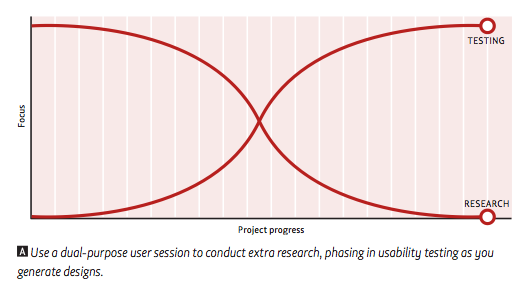
\includegraphics[width=0.6\linewidth]{images/bowles_dualpurpose_testing.png}}
  \end{center}
  \caption{User session focus chart published in ``Undercover User Experience Design'' \cite{bowles2011undercover}}
  \label{bowles_dualpurpose_chart}
\end{figure}

\subsubsection{With students}

In the meetings with students, the questions asked predominantly revolved
around module allocation at the University of York; it was important to
understand how students feel about the current state of module allocation to
ensure that this system improves their experience.

Students were asked to use a mockup of the application written in \gls{html}
and the researcher observed them to discover the main sources of difficulty.
Students were asked how and where they access to web, to get an understanding
of the environments this application might be used in.

During the implementation phase of the project, focus groups organised by the
\gls{aso} were conducted with students from each of the pilot departments.
\gls{lc} discussed with the students their current understanding of module
allocation, and their feelings on where it worked well and how it could be
improved. The project implementer tested several mockups of the student
interface by asking the students to visit hyperlinks. After the students had
the chance to use the mockups in a University computer classroom, they were
provided refreshments and took part in a discussion to gather their feedback.

In the History student focus group (eight students from 1st to 3rd year), it
was immediately clear that the two-column drag-and-drop layout
(Figure~\ref{prototype_student_2col}) was the easiest to use and related to
students' existing mental model most closely. As one student at the focus
group commented, this interface closely resembles the way in which the
\gls{yusu} website allows students to vote for sabbatical officers during
their annual elections. As students will already have some (however minimal)
experience with this kind of interface it makes sense to reuse ideas they are
used to.

Students were pleased with the simple drag-and-drop single column prototype,
but preferred the more explicit action of dragging from one side of the page
to the other. The weighting based system (dragging horizontal bars) was
unpopular with the History students; they commented that it would be
advantageous to have a simple system that all students can understand easily,
rather than one which may cause confusion -- especially when students are
preoccupied with making their module choices and do not want to think about
the way in which the system works.

In the Archaeology student focus group (six students from 1st to 3rd year),
similar concerns were raised about the second mockup. The students wondered
how the system would react if a only one or two modules were weighted
incredibly heavily and the remaining modules equally lightly. This is a
concern that would have to be discussed with the departments in depth and
communicated clearly to students in order to come up with an allocation that
was understood by all.

The students again commented on the similarity between the \gls{yusu} website
and the second mockup, reinforcing the previous group's feedback that this
mockup was the best of the three.

With this group of students, it was easy to observe a common issue of running
focus groups. Two of the Archaeology students present were more quiet than the
others in the group and it was harder to get their opinions. The solution in
this case was to direct specific questions at those two students, though
obviously this was not ideal. If running the session again, it would be
advantageous to not include those students in the focus group and instead
gather their opinions without the other students present.

\subsubsection{With staff}

Information was gathered from staff at the project steering group meetings and
at individual consultation sessions with each of the pilot departments.

It was mentioned at the first group meeting that previous systems used by
departments had been far too complicated for what departments required. A
departmental administrator commented that simplicity would be far more useful.

Staff raised the issue of what would happen to students who did not bother to
use the system to indicate a preference. It was decided that these students
could be randomly allocated, but that departments should be made aware which
students had been randomly allocated so that they could verify the
allocations. Related to this, departments required that they were able to send
out reminder emails to students who had not used the software.

More specific requirements started to come to light from mid-October, as staff
began to think more about the software and discuss it with colleagues.
\gls{sa} requested that some form of capability for human intervention should
be included in the software, to allow the departments to improve the allocation
once it had been made automatically.

On the issue of fairness, both departments were able to quantify their
allocation successes in previous years by saying ``no student was allocated a
module which was below their $n^{th}$ choice'' (where $n$ is different for
each department). The only other information obtained was that it would be
beneficial to keep the tail of students shorter -- that is, the software should attempt
to minimise the number of students who receive very bad allocations, if
possible.

I met with \gls{mh}, a member of \gls{ssdt}, to ascertain the format that
departments would provide the data to make the \gls{sits} import as easy as
possible.

It quickly became apparent that a table in which each row was a single
allocation (a \studmod pair) would allow the
team to import the data easily. It was agreed that the following information
would be provided for each allocation:

\begin{itemize}
  \item Student information: University username, \gls{routecode}, \gls{stage}
  \item Module information: module code, number of credits, which term the module is running in
\end{itemize}

Other information was added to accompany the data as it is being imported, but it
consisted of simply static values and was purely for convenience (such as the
letter \texttt{O} to indicate optional).

